\documentclass[a4paper,10pt,oneside,reqno]{scrartcl}
\usepackage[utf8]{inputenc}
\usepackage{listingsutf8}
\usepackage[pdftex]{graphicx}
%\usepackage[ngerman]{babel}
\usepackage{url}
\usepackage{hyperref}
\usepackage{amsfonts}
\usepackage{amssymb}
\usepackage{amsmath}
\usepackage{tikz}
\usepackage{listings}
\usepackage{pdfpages}
\usepackage{textcomp}
\usepackage{amsmath}
%\usepackage{lipsum}%%%%%%%%%%%%%%%%%%%%%%%%%%%%%%%%%%%%%%%%%%%%%%%%%%%%%%%%%%%%%%%%%%%%%%%%%%%%%%%%%%%%
\usepackage{mathtools}
\usepackage{amsfonts}
\usepackage{amssymb}
\usepackage{amsmath}
\usepackage{booktabs}
%usepackage[utf8x]{inputenc}
\usepackage[T1]{fontenc}
\usepackage{lmodern} %Latin modern = enhanced CM font
\usepackage{xspace} %Space enhancements
%\usepackage{algorithmic}%%%%%%%%%%%%%%%%%%%%%%%%%%%%%%%%%%%%%%%%%%%%%%%%%%%%%%%%%%%%%%%%%%%%%%%%%%%%%%%%%%
%\usepackage{algpseudocode}

%opening
\title{Übungsblatt 4}
\author{Uli Köhler (10580373), Tobias Harrer (10575835)}
\begin{document}

\maketitle
\section*{Aufgabe 1}%U
Siehe weiter unten, nach Aufgabe 4.

\section*{Aufgabe 2}%U
\paragraph{Datenstruktur:}
Die Datenstruktur sei eine verlinkte Liste von dynamisch erweiterbaren Arrays, z.B. \textit{LinkedList<LinkedList<Char> > alignments} in Java.
Die (äußere) verlinkte Liste enthält die einzelnen, durch Gaps unterbrochenen Alignments, die durch Strings unterbrochen werden. Zudem wird eine Liste an noch zu iterierenden Baumknoten angegeben, z.B. \textit{LinkedList<Node> unprocessedNodes}. Außerdem wird eine Assoziative Struktur zur Zuordnung von einem Knoten zur diesem Knoten entsprechenden Sequenz (\textit{ArrayList<Char>} die in der oben genannten Sequenzliste enthalten ist) gespeichert, z.B. in Java \textit{HashMap<Node, ArrayList<Char> > nodeToAlignmentSequence}. Wichtig ist hier, dass die Werte dieses Mappings auf dieselben Instanzen wie oben verweisen.

Das Alignment wird nun wie Folgt erstellt, sei $n$ die Anzahl der Sequenzen und $k$ die maximale Länge der Sequenzen: 

Über den gegebenen Baum wird wie folgt iteriert:
\textbf{Prozedur A} Für den aktuellen Knoten (Start: Wurzelknoten) werden alle Kindknoten aufgelistet (hat der Knoten keine Kindknoten, wird die Prozedur sofort beendet). Jeder dieser Kindknoten wird an die Liste der noch zu iterierenden Knoten angefügt. Es ergeben sich nun Paare aus dem aktuellen Knoten und einem Kindknoten. Ist die Liste an Alignments leer (d.h. ist der aktuelle Knoten der Wurzelknoten), so wird an die Liste der Alignments die Sequenz des Wurzelknotens angefügt und in \textit{nodeToAlignmentSequence} der Eintrag \textit{Wurzelknoten \textrightarrow eben in alignments eingefügte Sequenz} eingefügt. Für jedes Paar aus aktuellem Knoten und seinem Kindknoten wird nun die Prozedur B ausgeführt. Zudem werden alle Kindknoten an \textit{unprocessedNodes} angefügt. Der erste Knoten aus \textit{unprocessedNodes} wird nun entfernt und Prozedur A für diesen Knoten (als aktuellen Knoten) ausgeführt, bis \textit{unprocessedNodes} leer ist (\textrightarrow Termination).\\[5mm]

\textbf{Prozedur B}. Eingabe: Paar aus Elternknoten $k_e$ und Kindknoten $k_k$. Dein beiden Knoten seien im Baum die Sequenzen $s_a$ und $s_b$ zugeordnet. Zuerst wird für diese beiden Sequenzen eine optimales paarweises Alignment berechnet $\mathcal{O}(n^2)$. Aufgrund der vorhergehenden Schritte ist bekannt, dass sich die Sequenz des Elternknotens bereits in \textit{alignments} und auch in in \textit{nodeToAlignmentSequence} vorhanden ist -- das Alignment für $s_e$ ist  	. Für jedes Zeichen des soeben berechneten paarweisen optimalen Alignments wird nun wie folgt vorgegangen:

Wurde in die Sequenz $s_e$ beim paarweisen Alignmenteine Gap eingefügt, so wird in alle Alignments (\textrightarrow $\mathcal{O}(k)$ an der entsprechenden Position eine Gap eingefügt. Ansonsten wird das Zeichen an der entsprechenden Position im paarweisen Alignment von $s_k$ übernommen.

Danach wird für alle Positionen, an denen das Alignment für $s_e$ bereits eine Gap enthielt, auch in das Alignment der Kindsequenz eine Gap eingefügt. Das resultierende Alignment wird nun an \textit{alignments} angefügt und das Mapping \textit{nodeToAlignmentSequence} wird entsprechend upgedated.

\textbf{Einstiegspunkt} Am Anfang wird Prozedur A mit dem Wurzelknoten als aktuellem Knoten ausgeführt.

\textit{Korrektheit} Die Korrektheit wurde bereits im Skript bewiesen.

\textit{Termination} Da nur die Kindknoten in die Liste \textit{unprocessedNodes} eingefügt werden, und bei einer Iteration der Prozedur A einer der Knoten aus der Liste entfernt wird, wird Prozedur A für jeden Knoten im Baum genau einmal ausgeführt. Da Bäume \textit{per definitionem} keine Loops haben dürfen, wird Prozedur A für jeden Knoten genau einmal ausgeführt.

\textit{Laufzeit}
Die Folgenden Faktoren spielen eine Rolle für die Laufzeit (Hinweis: Insertion aus Sicht von $s_e$, d.h. Gap ist auf $s_k$):
\begin{itemize}
 \item Das Einfügen in die Listen bzw. Maps sowie das Abrufen der Alignment-Referenz für einen gegebenen Knoten wird als konstant angenommen. Einige mögliche Implementierungen, die z.B. immutable Strings als Alignments nutzen, haben allerdings eine $\mathcal{O}(k)$-Laufzeit für einige Operation. Es wird nicht davon ausgegangen, dass der Programmierer eine solche suboptimale Ausprägung implementiert.
 \item Prozedur A wird für jede Sequenz exakt einmal ausgeführt (siehe auch Terminationsbeweis), benötigt (abgesehen von der Ausführung von Prozedur B) aber konstante Laufzeit
 \item Prozedur B wird (n-1) mal ausgeführt, da es nicht für den Wurzelknoten, aber aufgrund der Baumstruktur für alle anderen Knoten genau ausgeführt wird
 \item Die Berechnung eines optimalen paarweisen Alignments benötigt $\mathcal{O}(k^2)$ Zeit, wobei insgesamt (selbe Argumentation wie bei Proz. B) (n-1) Alignments ausgeführt werden.
 \item Für jede Deletion/Substitution im paarweisen Alignment wird konstante Zeit benötigt
 \item Für jede Insertion im paarweisen Alignment wird $\mathcal{O}(n)$ Zeit benötigt
 \item Da das paarweise Alignment max. $2k$ lang ist, d.h. $\mathcal{O}(k)$ wird maximal $\mathcal{O}(k*n)$ Zeit (wenn das Alignment nur aus Insertionen besteht
 \item Eine Ausführung von Prozedur B benötigt also im Worst Case $\mathcal{O}(k^3*n)$ Zeit.
 \item Da Proz. A konstante Zeit benötigt, und Proz. B wie oben gezeigt (n-1) mal ausgeführt wird, benötigt die gesamte Prozedur max. $\mathcal{O}(k^3*n^2)$ Zeit.
\end{itemize}

\section*{Aufgabe 3}%T
Als erstes muss das Zentrum des Baums/Sterns gefunden werden. Nach Def. 6.36 ist der Center-String $s_c$ 
so zu wählen, dass $\Sigma_{j=1}^k d(s_c, s_j)$ minimal ist. Für die gegeben Sequenzen ergeben sich
zusammen mit den zugehörigen Distanzen folgende Summen:
\begin{enumerate}
 \item $\Sigma_{j=1}^4 d(s_j, s_1) = 0 + 3 + 3 + 3 = 9$
 \item $\Sigma_{j=1}^4 d(s_j, s_2) = 3 + 0 + 2 + 4 = 9$
 \item $\Sigma_{j=1}^4 d(s_j, s_3) = 3 + 2 + 0 + 3 = 8$
 \item $\Sigma_{j=1}^4 d(s_j, s_4) = 3 + 4 + 3 + 0 = 10$
\end{enumerate}
Daraus folgt, dass $s_3$ die geringste Distanz zu allen anderen Sequenzen hat. Mit meiner GoBi-
Implementierung (/home/proj/biocluster/praktikum/genprakt-ws13/abgaben/assignment1/harrer/gotoh.jar) bekomme ich die folgenden Alignments:\newline
\texttt{
s3: CAATG\newline
s1: CGA-A\newline\newline
s3: CAATG-\newline
s2: CAGTGA\newline\newline
s3: C-AATG\newline
s4: CGGATT\newline}

Gemäß dem Hinweis aus der letzen Übungsbesprechung wird das MSA schrittweise vom Zentrum aus aufgebaut.
\texttt{s3: CAATG\newline
s1: CGA-A\newline\newline
s3: CAATG-\newline
s1: CGA-A-\newline
s2: CAGTGA
\newline\newline
s3: C-AATG-\newline
s1: C-GA-A-\newline
s2: C-AGTGA\newline
s4: CGGATT-}

\section*{Aufgabe 4}%T
Annahme: $M(\lfloor \frac{k+1}{2}\rfloor) > 3M$, also soll die kummulierte Distanz der Sequenz $s_{\lfloor \frac{k+1}{2}\rfloor}$
$M(\lfloor \frac{k+1}{2}\rfloor) = \Sigma_{j=1}^k d(s_{\lfloor \frac{k+1}{2}\rfloor}, s_j)$ zu allen anderen Sequenzen größer als
das dreifache von $M$ sein, wobei nach Def. $M = M(1)$ ist.
Nach Lemma 6.50 gibt es mehr als $\lfloor \frac{k}{r}\rfloor$ Sequenzen $s_i \in S$, wobei der Konsensus-Fehler von $s_i$ kleiner gleich
$\frac{2r-1}{r-1}*E_S(s*)$ ist, wobei $1<r \in \mathbb{R}$. Da $r$ echt größer als 1 ist, gibt es mindestens zwischen 0 und $k-1$ Sequenzen,
die die Ungleichung aus 6.50 erfüllen, da $\lfloor \frac{k}{r+\epsilon}\rfloor \leq k-1$  $\forall$  $\mathbb{R} \ni \epsilon > 0$ und
$\lfloor \frac{k}{r}\rfloor \geq 0$ $\forall$ $r>k$.\newline
Ist $r$ nahe der 1, dann gibt es mehr als $k-1$ Sequenzen $s_i \in S$, deren Konsensus-Fehler kleiner gleich $\frac{2r-1}{r-1}*E_S(s*)$ ist,
wobei der Vorfaktor immer größer wird, je näher $r$ gegen 1 geht. Im anderen Fall, wenn $r>k$ ist, dann konvergiert der Vorfaktor
asymptotisch gegen 2, das heißt es gibt mehr als 0, also mindestens eine Sequenz $s_i \in S$, deren Konsensusfehler höchstens doppelt so hoch
ist wie der minimale Konsensusfehler.\newline
Angenommen $r=2$, dann gibt es \textit{mehr als} $\lfloor \frac{k}{2}\rfloor$ Sequenzen $s_i \in S$ mit $E_S(s_i) \leq \frac{2*2-1}{2-1}*E_S(s*)
= 3*E_S(s*)$. Da der sog. Steiner-String s* diejenige Zeichenreihe $\in \Sigma^*$ ist, die den geringsten Konsensusfehler hat, kann man davon
ausgehen, dass $E_S(s*) \leq M := M(1)$ ist.
Angenommen $M(\lfloor \frac{k+1}{2}\rfloor) > 3M$, dann stellt dies einen Widerspruch zu Lemma 6.50 dar, denn:\newline
In diesem Fall gibt es also gemäß Lemma 6.50 \textit{mehr als} $\lfloor \frac{k}{2}\rfloor$ Sequenzen, deren Konsensusfehler $\leq 3*E_S(s*)$ sind, und gemäß
der Widerspruchs-Annahme gilt gleichzeitig, dass die kummulierte Distanz der  $\lfloor \frac{k+1}{2}\rfloor$-ten Sequenz zu allen anderen
Sequenzen $>3*M \geq 3*E_S(s_i)$ ist, was nicht sein kann. Denn in diesem Fall kann es nicht mehr als $\lfloor \frac{k}{2}\rfloor$ Sequenzen
geben, deren Konsensusfehler $\leq 3*E_S(s*)$  ist, da die $\lfloor \frac{k+1}{2}\rfloor$-te Sequenz bereits einen Konsensusfehler von
mehr als $3*M$ hat, und wir von der Widerspruch-Annahme ausgehen.\newline
Also folgt $M(\lfloor \frac{k+1}{2}\rfloor) \leq 3M$, was zu zeigen war.

\section*{Aufgabe 1}%U
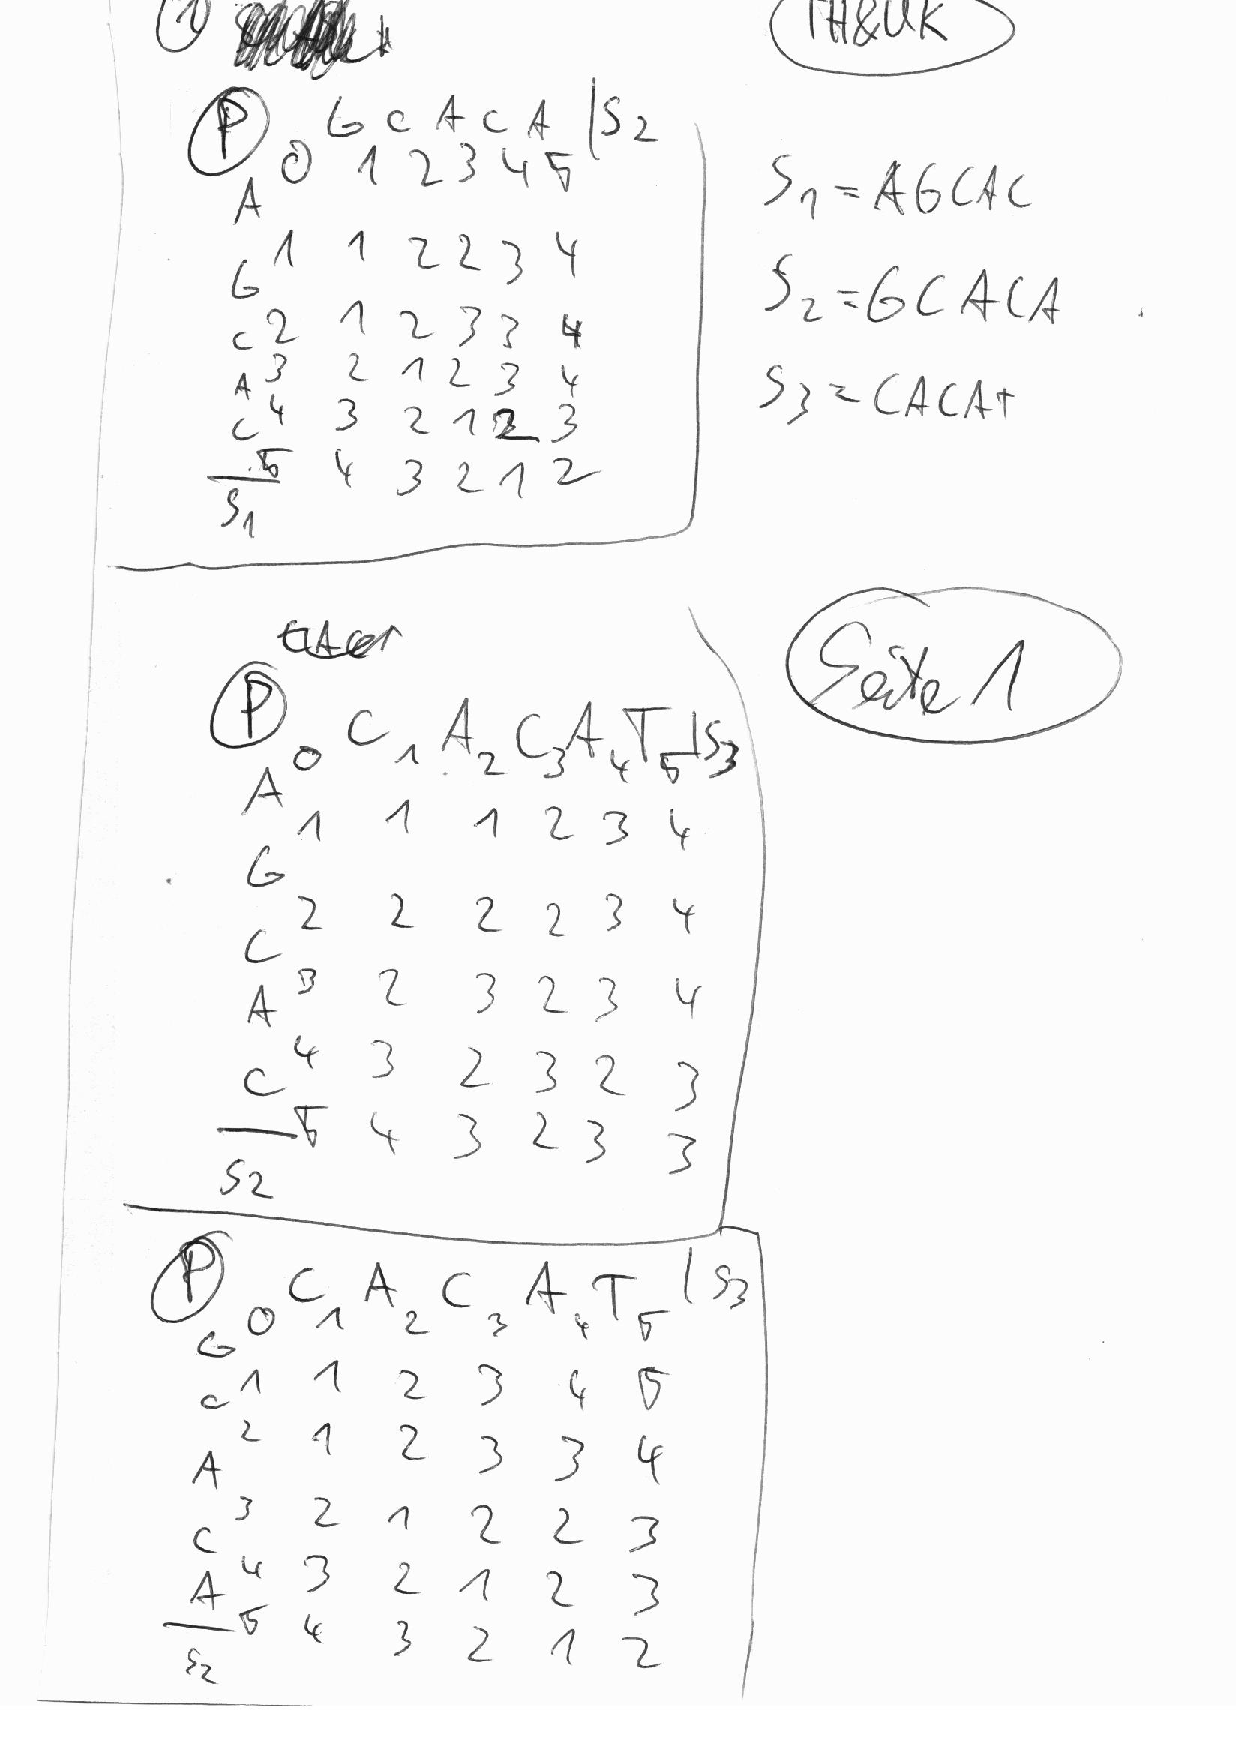
\includepdf[pages=1]{1.pdf}
\includepdf[pages=2]{1.pdf}
\includepdf[pages=3]{1.pdf}
\includepdf[pages=4]{1.pdf}
\includepdf[pages=5]{1.pdf}
 
\end{document}
